%% mascots.tex

% TODO Major:
% * Make it apperent that the paper studies the performance of accelerated
%   graphics on a platform using virtualization hardware extensions to speed up
%   execution on x86. Accentuate why it is probable that x86 is not the target
%   platform, and that the solution would probably speed up graphics by orders
%   of magnitude more should virtualization extensions not be used.
% * Briefly mention that OpenGL ES 2.0 is chosen because it's often used for
%   embedded platforms (which is one of Simics' strenths).
% * The section on GPU Modeling can probably be shortened quite a bit. Consider
%   breaking out the contents of the subsections under the overhead title.
% * Consider placing the section on OpenGL Framework Generation after
%   descriptions of target and host libraries.
% * I've commented out descriptions on the setup of the QEMU Android
%   emulator from the Experimental Methodology section. Consider
%   adding them to the document if we're to expand on the comparisons
%   with the android emulator.
% * The Platform Comparison section (commented out under Methods and Results)
%   should probably be uncommented and moved to a later section if we want to
%   bring up QEMU.
% * Explain in detail why paravirtualization is a good balancing of
%   the problems facing graphics acceleration in system simulation.
% * Refer to the benchmarks, not at Chess or Julia, but as the 'latency' and
%   'compute'/'performance' (?) benchmarks.
% * The benchmarks are open source. Reference the repository.
% * Explain Future Work?
% * Merge the Target and Host system libraries sections.
% * Merge the Simics Pipe and page table traversal sections.
% * The 'read-first-line-from-file'-command seems to carry about some
%   unnecessary whitespace with it. Remove. When this has been done, it is
%   plausible that the tables may be put side-by-side.

% TODO Minor:
% * Correct formatting of multiple references [4][34] -> [4,34].
% * Indentation at the start of sections.

% Thesis chapters yet to import contents from:
% * Discussion (?)
% * Future work (consider adding some future work bits)

\documentclass[conference]{IEEEtran}
% If IEEE MASCOTS is part of the IEEE Computer Society- range of
% conferences, be sure to add the compsoc option to the document class.
% If IEEEtran.cls has not been installed into the LaTeX system files,
% manually specify the path to it like:
%\documentclass[conference]{../sty/IEEEtran}

\usepackage{soul} % Used to temporarily highlight areas of text during writing.
\usepackage{xcolor} % colorbox for the inline code command.
\usepackage{hyperref} % Hyperlinks and urls.
\usepackage{listings} % code boxes.
\usepackage{amsfonts} % \circledR.
\usepackage{graphicx} % Displaying pdf graphics.
\usepackage{multirow} % Used for specialized tables (multirow).
\usepackage{rotating} % Used to rotate figures sideways.
\usepackage{todonotes} % Used to add TODOs in the document. Remove when no longer needed.
\usepackage[mediumspace,mediumqspace,squaren,binary]{SIunits} % \milli\second

% correct bad hyphenation here
\hyphenation{op-tical net-works semi-conduc-tor}

% These should probably be merged into the same bibliography list in
% the end, but it might be good to have them seperately now so that
% it's easier to filter out possibly unreliable sources.  When most
% contents have been imported from the thesis, replace these with
% suitable commands.
\newcommand{\dvtcmdcitebib}[2][]{\cite{#2}} % TODO: \masccitebib
\newcommand{\dvtcmdciteref}[2][]{\cite{#2}} % TODO: \mascciteref
%\newcommand{\dvtcmdcitefur}[2][]{\citefur{#2}}
\newcommand{\dvtcmdrefname}[1]{\nameref{#1}}

% Formatting inline code command:
\newcommand{\dvtcmdcodeinline}[1]{\colorbox{black!5}{\lstinline[basicstyle=\ttfamily\color{black}]{#1}}}
% Command to read, and ouput the first line of a file:
\newread\file
\newcommand{\dvtcmdfirstline}[1]{\input{#1}\unskip}

\begin{document}

\title{%
  Accelerating Graphics in\\
  the Simics Full-system Simulator}

\author{\IEEEauthorblockN{Eric Nilsson\IEEEauthorrefmark{1},
    Daniel Aarno\IEEEauthorrefmark{2}, and Erik Carstensen\IEEEauthorrefmark{3}}
  \IEEEauthorblockA{Intel Corporation\\
    Stockholm, Sweden\\
    Email: \IEEEauthorrefmark{1}\href{mailto:eric.nilsson@intel.com}{eric.nilsson@intel.com},
    \IEEEauthorrefmark{2}\href{mailto:daniel.aarno@intel.com}{daniel.aarno@intel.com},
    \IEEEauthorrefmark{3}\href{mailto:erik.carstensen@intel.com}{erik.carstensen@intel.com}}
  \and
  \IEEEauthorblockN{Prof. H{\aa}kan Grahn}
  \IEEEauthorblockA{Blekinge Institute of Technology\\
    Karlskrona, Sweden\\
    Email: \href{mailto:hakan.grahn@bth.se}{hakan.grahn@bth.se}}}

\maketitle

\begin{abstract}
Virtual platforms provide benefits to developers in terms of a more rapid development cycle since development may begin before next-generation hardware is available.
However, there is a distinct lack of graphics virtualization in industry-grade virtual platforms, leading to performance issues that may reduce the benefits virtual platforms otherwise have over execution on actual hardware.

This paper demonstrates graphics acceleration by the means of paravirtualizing OpenGL~ES in the Wind~River Simics full-system simulator.
We propose a solution for paravirtualized graphics using magic instructions to share memory between target and host systems, and present an implementation utilizing this method.
The study illustrates the benefits and drawbacks of paravirtualized graphics acceleration and presents a performance analysis of strengths and weaknesses compared to software rasterization.
Additionally, benchmarks are devised to stress key aspects in the solution, such as communication latency and computationally intensive applications.

We assess paravirtualization as a viable method to accelerate graphics in system simulators; this reduces frame times up to 34 times compared to that of software rasterization.
Furthermore, magic instructions are identified as the primary bottleneck of communication latency in the implementation.
\end{abstract}

% Introduction
\section{Introduction}
\label{sec:introduction}
Virtual platforms are becoming an important tool in the software industry in order to provide cost-effective time-to-market gains and meet the ever-shortening product life-cycles~\masccite{journals:magnusson:2002, journals:yi:2006, publications:leupers:2010, publications:aarno:2014}.
Virtual platforms deliver these time-to-market benefits by enabling pre-silicon development~\masccite[p.~52]{journals:magnusson:2002, publications:aarno:2014} and by providing tools such as deterministic execution, checkpointing, and reverse execution~\masccite{publications:aarno:2014, journals:aarno:2013}.
These features are useful for debugging and testing a diverse range of software, from firmware to end-user applications~\masccite[p.~25]{publications:leupers:2010}.

There are several techniques to provide fast and functional virtual platforms that are running CPU workloads.
Typical methods include interpretation~\masccite[p.~35]{journals:smith:2005, inproceedings:magnusson:1998}, just-in-time compilation~\masccite[p.~24,~25]{journals:aarno:2013, inproceedings:magnusson:1998}, and hardware-assisted virtualization~\masccite[p.~24,~25]{journals:aarno:2013, publications:leupers:2010}.
Virtual platforms using these techniques can typically achieve a simulation performance in the range of $10$-$1000$ million instructions per second~\masccite[p.~24,~25]{journals:aarno:2013}.

The GPU is a vital part in delivering good user experiences on many devices, ranging from wearable, hand held, and portable units, to desktop computers.
The widespread use of GPUs and the increasing complexity of these electronic systems extend the virtualization needs of such devices.
However, due to large architectural differences, delegating GPU workloads to CPUs may yield poor performance.

Instead, by neglecting some hardware compatibility, one may circumvent the virtual machine and delegate GPU workloads to the GPU of the simulation host.
This way, host hardware can be utilized in a process known as "Paravirtualization"~\masccite[p.~1]{inproceedings:youseff:2006}.
Paravirtualization has been used to accelerate graphics in the past; most notably, Lagar-Cavilla et al. accelerate OpenGL~$1.5$ up to two orders of magnitude for WMware~Workstation and Xen VMMs~\masccite{inproceedings:lagarcavilla:2007}.
To relieve communication bottlenecks, Lagar-Cavilla et al. suggests using a shared memory model for target-to-host communications~\masccite{inproceedings:lagarcavilla:2007}.

This paper presents the acceleration of OpenGL~ES~$2.0$ in the Simics full-system simulator, using magic instructions to share VM memory directly from a simulated RAM image.
The implementation is evaluated using performance benchmarks stressing important attributes of the devised solution, and subsequently compared to software rasterization on the simulated platform.
Furthermore, the study identifies performance bottlenecks that may obstruct paravirtualized real-time graphics.
The results presented in this paper show performance improvements of up to $34$ times compared to software rasterized counterparts.

% previousresearch.tex

% Previous Research
\section{Previous Research}
\label{sec:previousresearch}

\ldots

% problemformulation.tex

% Problem Formulation
\section{Problem Formulation}
\label{sec:problemformulation}
The study presented in this document consists of implementing paravirtualization of a graphics API (being OpenGL~ES~$2.0$ ) in the Simics full-system simulator developed by Intel\circledR and sold through Intel\circledR 's subsidiary Wind River Systems, Inc. 
The solution devised to accelerate OpenGL adheres to that of the Android emulator, which is elaborated upon in section \ref{sec:previousresearch_qemu}.
As such, this study concerns investigating the performance, and the feasibility of extended benefits and advanced functionality, of paravirtualized graphics in a virtual platform.
This entails investigation, analysis, and development of methods and techniques for efficient communication and execution in the Simics run-time environment.
Furthermore, the study comprises analysis of the liabilities of paravirtualized technologies in regards to Simics philosophy (being high-performance determinism and repeatability~\dvtcmdcitebib{journals:aarno:2013}).
Thus, the study does not exclusively concern Simics integration, but an investigation of paravirtualized libraries in virtual platforms.

For the purpose of this paper, a paravirtualized solution for graphics acceleration in Simics is developed.
Furthermore, to accommodate the analysis of benefits and drawbacks of paravirtualized graphics, a number of benchmarks are devised to stress key points in the developed solution; with the goal of locating performance bottlenecks.
The benchmarks are designed to stress latency and bandwidth in target -to-host communication, in addition to computational intensity brought on by complex GPU -bound workloads.

Based on the devised solution, in coagency with the benchmarks, this study comprises an analysis of the performance of paravirtualized graphics compared to that of traditional software rasterization.
The objectives of the paper is to evaluate the feasibility of paravirtualization as an approach to accelerate graphics in virtual platforms; along with identifying its strengths and weaknesses.

In line with previous work in the area specified in chapter \ref{cha:previousresearch}, there has been no indication - in academic writing - of any pre-existing solution of paravirtualized graphics APIs signifying deterministic behavior; paving the way for supporting reverse execution graphics.
Such functionality could simplify debugging, testing, and profiling of applications comprising some GPU -bound workload; not limited to graphics- or GPU utilization in its entirety.
Entailed by these research gaps, the research questions formulated in this chapter are considered to be lacking in the field.

As such, the study performed for the purposes of this paper is relevant to the field of computer science by expanding upon the the knowledge of graphics acceleration in virtual platforms; in terms of facilitating debugging, testing, and profiling of software dependent on GPU graphics acceleration.
By the means outlined in chapter \ref{cha:aimsandobjectives}, this paper contributes to the field of computer science by answering these questions from the perspective of graphics paravirtualization in the Simics full-system simulator.
Accordingly, the key investigatory attributes and explicit research question formulations, sought to be answered by this paper, are presented below.

\newcommand*\researchquestionitem[2]{\item[#1:] \textit{#2}}
\begin{itemize}[noitemsep]
	\researchquestionitem{1}{What constitutes a viable implementation of paravirtualized graphics?}
	\researchquestionitem{2}{What are the benefits and disadvantages of paravirtualized graphics?}
	\researchquestionitem{3}{How does paravirtualized graphics performance relate to software rasterization?}
\end{itemize}

Furthermore, the study pertains to a number of discussion topics in line with the solution's relation to the Simics full-system simulator. These discussion questions presented below.

\begin{itemize}[noitemsep]
	\researchquestionitem{1}{What inhibits deterministic execution of paravirtualized graphics?}
	\researchquestionitem{2}{What inhibits checkpointing of paravirtualized graphics?}
	\researchquestionitem{3}{What inhibits reverse execution of paravirtualized graphics?}
\end{itemize}

% methodsandresults.tex

\begin{figure}
\setlength{\abovecaptionskip}{0pt}
\setlength{\belowcaptionskip}{0pt}
\centering
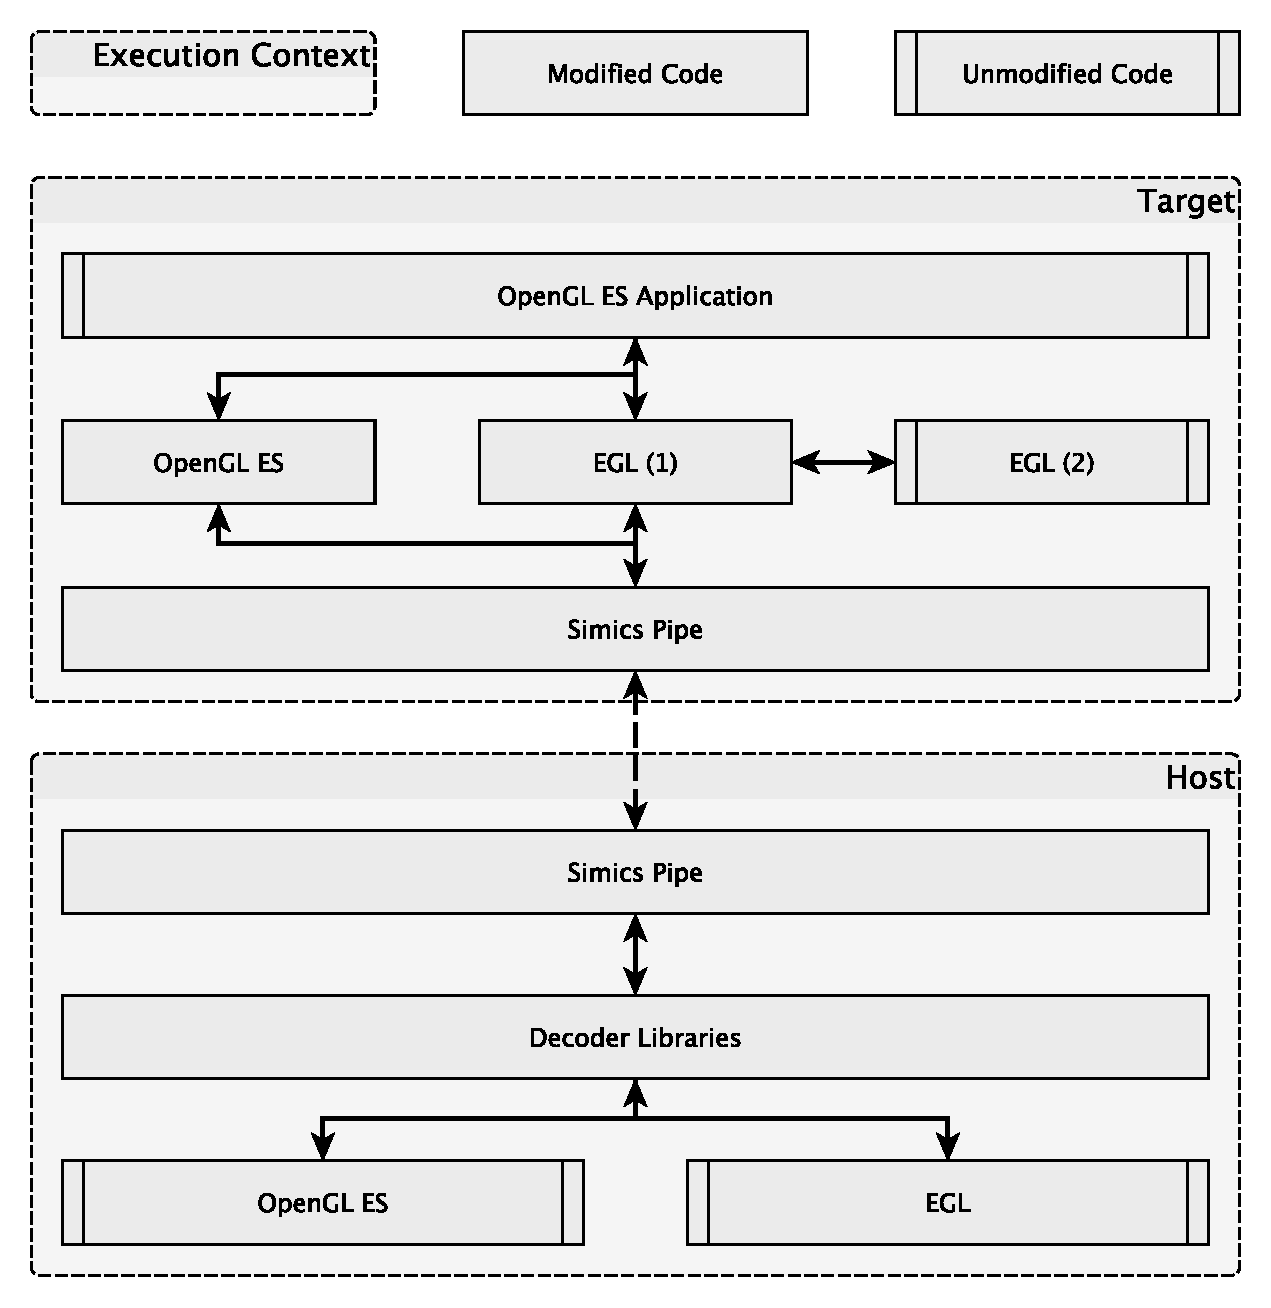
\includegraphics[width=\linewidth]{img/yedoverview.pdf}
\caption{Overview of paravirtualized graphics in Simics.}
\label{fig:overview}
\end{figure}

% Methods and Results
\section{Methods and Results}
\label{sec:methodsandresults}
OpenGL paravirtualization in Simics encompasses three overall components, being the target system libraries, the host system libraries, and a communications channel between them named the "Simics pipe".
To facilitate easier development, target and host system libraries may be partly generated from specification files detailing function signatures and arguments.
Except methods that require state saving, the majority of the libraries are generated this way.

The target system libraries implement the OpenGL and EGL (the interface between OpenGL and the underlying platform windowing system) APIs; unmodified binaries in the target system are subsequently linked with these libraries as with any other OpenGL or EGL implementation.
However, instead of communicating with the graphics device, the target system libraries serialize and forwards the command stream to the simulation host.
The transmission is not necessarily performed at once, or in the designated order, because of uncertainties regarding argument data proportion.
For instance, the number of vertices to be rendered does not have to be apparent at a given time, but implicit in a later OpenGL invocation.
Accordingly, certain function calls have to be delayed until more information is known about the OpenGL state.

In collaboration with the target system libraries, the host system libraries decodes and interprets the received byte stream.
Subsequently, the host system libraries may safely perform the relayed workload and return any results to the target system.

Both target and host system libraries maintain a subset of the OpenGL state, such as bound vertex buffers and attribute properties.
These states must be maintained because of the asynchronous nature of the command stream.

Because of differences in the creation and maintenance of windows on different platforms (Fedora, Android, etc.), the window to which OpenGL renders is kept on the simulation host.
This is problematic; the target system libraries must communicate with a fraudulent window in the simulation host -- \textit{and} the native window.
For example, it is important that the native window reports successful initialization, lest the OpenGL application concludes an error and quits.
The issue is overcome by selectively overriding symbols in the target libraries so that a subset of functions may be overloaded.
This way, one may extend the original EGL library to invoke the simulation host prior to performing its actions.

To communicate with the simulation host, the Simics pipe uses "magic instructions".
Magic instructions denotes \masccodeinline{nop}-type instructions that, when executed on the simulated hardware in a virtual platform, invoke a callback-method in the simulation host~\masccite[p.~32]{publications:leupers:2010}.
Because of the inherent performance demands brought on by real-time graphics, they constitute a suitable communications medium for rendering information between target and host systems.

During a magic instruction, we may utilize any available registers; the number and size of registers is the data-sharing bottleneck of this method.
Thus, we transmit the starting address of the serialized command stream in a 64-bit register.
Having escaped the simulation context, Simics can translate the transmitted virtual address to a physical one using the virtual machine MMU.
Consequently, the physical address can be used to locate the memory page in the simulated RAM image.
To ensure the pages are not swapped to disk when the simulation state is paused, we "lock" all pages constituting the command stream buffer.
Subsequently, all memory pages are continiously retrieved by iterating the original virtual address with the target page size, effectively 'traversing' the virtual memory table.

\subsection{Experimental Methodology}
\label{sec:experimentalmethodology}
To evaluate the implementation, performance of paravirtualized graphics in Simics is compared to software rasterization.
Simics itself simulates an Intel\circledR ~Core\texttrademark ~i7 processor and an Intel\circledR ~X58 chipset.
Throughout simulation, hardware-assisted virtualization using KVM runs x86 instructions natively on the host hardware.
Like the host system, the simulation target runs Fedora~$19$ Linux and use the Mesa llvmpipe driver software rasterizer~\masccite{web:mesa:2015}.

The experiments are performed on a system with the following specifications:
\begin{itemize}
\item Intel\circledR\ Core\texttrademark\ i7-4770HQ
\item Intel\circledR\ Iris\texttrademark\ Pro Graphics 5200
\end{itemize}

Two benchmarks are devised on-site to stress suspected bottlenecks: one benchmark performs a large number of OpenGL invocations, while the other has a computationally intensive workload.
Given a target frame time of $16$~\milli\second , the benchmarks are configured to run at $10$ to $20$~\milli\second\ per frame, when hardware accelerated on the host system; a $16$~\milli\second\ frame time roughly corresponds to $60$~frames per second.
The benchmarks are shaped this way to reflect the expected load of a real-time interactive application.
As such, the benchmarks should be representative of typical scenarios induced by modern applications using OpenGL, such as responsive UIs.
The developed benchmark suite is open source and available online~\masccite{web:intel:2014}.

For each benchmark, the elapsed times of $1000$ frames are collected.
To gain some understanding on how well the given performance scales, three instances of each benchmark are run with smaller and larger input data, tuned to yield approximately half and double frame time..
The specifics of each benchmark are described below.

% Benchmark: Chess
\paragraph{Benchmark: Chess}
\label{par:experimentalmethodology_benchmarking_benchmarkchess}
The 'Chess' benchmark is developed for the purposes of stressing the latency between target and host systems.
It is so named because of the chess-like tile set the graphics kernel produces.
The benchmark is designed to perform a multitude of OpenGL invocations per frame, in which each invocation is relatively lightweight and carries a small amount of data in its arguments.
In the Chess benchmark, this is achieved by rendering a grid of tiles where each tile is represented by four two-dimensional vertices in screen-space, in addition to six indices outlining the rectangular shape.
Since the vertices are already transformed into screen-space, the graphics kernel does not need to perform any additional transformations.
Additionally, the tile set vertices and indices are pre-loaded into OpenGL vertex and index element buffers, so that a lone buffer identifier may be transmitted instead of the heavier vertex set load.
Each tile is then individually drawn to the back buffer, rendering the chess-like appearance of the benchmark.
Effectively, this means that, for each tile, the benchmark need only bind a vertex and an index element buffer, set the corresponding tile color, and lastly invoke the rendering of said tile.

For each frame rendered, depending on the number of drawn tiles, the solution will perform a large number of magic instructions.
This induces a high utilization of the Simics Pipe, which is intended to stress suspected magic instruction overhead.
The repeated invocation of lesser draw calls is representative of common usage of drawing a multitude of shapes with OpenGL, such as a UI.
As such, the benchmark is suitable for the purpose of representing a large number of graphics invocations.

We perform the Chess benchmark with $60\times60$, $84\times84$, and $118\times118$ tiles, which entails roughly $9\cdot60\cdot60$, $9\cdot84\cdot84$, and $9\cdot118\cdot118$ magic instructions per frame.

% Benchmark: Julia
\paragraph{Benchmark: Julia}
\label{par:experimentalmethodology_benchmarking_benchmarkjulia}
The 'Julia' benchmark is developed to stress computational intensity in the paravirtualized solution.
It is so named because the program calculates the Julia fractal~\masccite{web:tsiombikas:2014}.
The benchmark is designed to perform a lone, computationally intensive, invocation, which will stress the computational prowess of the profiled platform.
The case is selected for use as the computation of a fractal is trivially scalable in terms of complexity, by modifying the number of iterations the fractal algorithm performs.
Thus, it is suitable for profiling computationally intensive workloads.

We perform the Julia benchmark with $225$, $450$, and $900$ iterations per frame, all of which induce only $16$ magic instructions per frame.

\subsection{Threats to Validity}
\label{sec:threatstovalidity}
Because of complications caused by virtual time, profiling of elapsed time in simulators dictate special measures.
This is due to the fact that profiling of elapsed time outside of the simulation -- that is, time in the context of the observer -- may be more relevant than profiling of virtual time.
This is often the case if the simulation has outside dependencies of some sort.
Naturally, it is so in terms of real-time interaction and rendering.

In order to profile elapsed frame times, profiling must take place outside of the simulation.
One way of achieving this is to listen in on activity passing through a target serial port; this is a traditional front-end to the machine.
In this way, the simulator is instructed to listen in on, and set a simulation breakpoint at the occurrence of, a specialized sequence of bytes being written to a UART serial port.
This is the method we use to profile frame time performance in Simics.

When using serial ports in this manner, one may introduce a profiling cost.
Such overhead may be induced because of file descriptors not immediately transmitting a concerned byte sequence via the system UART.
This overhead cost is measured to be, on average, $1.5$~\milli\second .
If not specified otherwise, presented results take into account the average of this profiling overhead.

\subsection{Results}
\label{sec:results}
Results accumulated from software rasterized and paravirtualized execution in Simics are presented in Tables~\ref{tab:keyvalsimics}~and~\ref{tab:keyvalpara}.
In Figure~\ref{fig:histogram}, the results are presented as histograms, visualizing elapsed time in milliseconds to sample density.
As such, the $Y$ axis illustrate the sample density.
For each experiment, the collected ($1000$) frame time samples are subdivided into $100$ bins.
For the purposes of visualization, values outside of the standard deviation are not featured in the figures.

The remainder of this section presents an analysis of the results.

\providecommand{\chesskeyone}{$60\times60$ tiles}
\providecommand{\chesskeytwo}{$84\times84$ tiles}
\providecommand{\chesskeythree}{$118\times118$ tiles}

\providecommand{\juliakeyone}{$225$ iterations}
\providecommand{\juliakeytwo}{$450$ iterations}
\providecommand{\juliakeythree}{$900$ iterations}

\begin{table*}
  \parbox{.5\textwidth}{
    % tab:keyvalsimics
    \centering
    \tabcolsep=0.11cm
    \begin{tabular}{|c|c|c|c|c|c|}
      \hline
      \multirow{2}{*}{Benchmark} & \multirow{2}{*}{Input} & \multicolumn{4}{p{4cm}|}{\centering Elapsed time (\milli\second )} \\
      \cline{3-6} && \multicolumn{1}{c|}{Min} & \multicolumn{1}{c|}{Max} & \multicolumn{1}{c|}{Std} & \multicolumn{1}{c|}{Avg} \\ \hline
      \multirow{3}{*}{Chess} & \chesskeyone & \mascfirstline{simicschess60x60.dat.min} & \mascfirstline{simicschess60x60.dat.max}	& \mascfirstline{simicschess60x60.dat.std} & \mascfirstline{simicschess60x60.dat.avg} \\ %\cline{2-6}
      & \chesskeytwo & \mascfirstline{simicschess84x84.dat.min} & \mascfirstline{simicschess84x84.dat.max} & \mascfirstline{simicschess84x84.dat.std} & \mascfirstline{simicschess84x84.dat.avg} \\ %\cline{2-6}
      & \chesskeythree & \mascfirstline{simicschess118x118.dat.min} & \mascfirstline{simicschess118x118.dat.max} & \mascfirstline{simicschess118x118.dat.std} & \mascfirstline{simicschess118x118.dat.avg} \\ \hline
      \multirow{3}{*}{Julia} & \juliakeyone & \mascfirstline{simicsjulia225.dat.min} & \mascfirstline{simicsjulia225.dat.max} & \mascfirstline{simicsjulia225.dat.std} & \mascfirstline{simicsjulia225.dat.avg} \\ %\cline{2-6}
      & \juliakeytwo & \mascfirstline{simicsjulia450.dat.min} & \mascfirstline{simicsjulia450.dat.max} & \mascfirstline{simicsjulia450.dat.std} & \mascfirstline{simicsjulia450.dat.avg} \\ %\cline{2-6}
      & \juliakeythree & \mascfirstline{simicsjulia900.dat.min} & \mascfirstline{simicsjulia900.dat.max} & \mascfirstline{simicsjulia900.dat.std} & \mascfirstline{simicsjulia900.dat.avg} \\ \hline
    \end{tabular}
    \caption{Software rasterization results in Simics.}
    \label{tab:keyvalsimics}
  }
  \hfill
  \parbox{.5\textwidth}{
    % tab:keyvalpara
    \centering
    \begin{tabular}{|c|c|c|c|c|c|}
      \hline
      \multirow{2}{*}{Benchmark} & \multirow{2}{*}{Input} & \multicolumn{4}{p{4cm}|}{\centering Elapsed time (\milli\second )} \\
      \cline{3-6} && \multicolumn{1}{c|}{Min} & \multicolumn{1}{c|}{Max} & \multicolumn{1}{c|}{Std} & \multicolumn{1}{c|}{Avg} \\ \hline
      \multirow{3}{*}{Chess} & \chesskeyone & \mascfirstline{parachess60x60.dat.min} & \mascfirstline{parachess60x60.dat.max} & \mascfirstline{parachess60x60.dat.std} & \mascfirstline{parachess60x60.dat.avg} \\
      & \chesskeytwo & \mascfirstline{parachess84x84.dat.min} & \mascfirstline{parachess84x84.dat.max} & \mascfirstline{parachess84x84.dat.std} & \mascfirstline{parachess84x84.dat.avg} \\
      & \chesskeythree & \mascfirstline{parachess118x118.dat.min} & \mascfirstline{parachess118x118.dat.max} & \mascfirstline{parachess118x118.dat.std} & \mascfirstline{parachess118x118.dat.avg} \\ \hline
      \multirow{3}{*}{Julia} & \juliakeyone & \mascfirstline{parajulia225.dat.min} & \mascfirstline{parajulia225.dat.max}	& \mascfirstline{parajulia225.dat.std} & \mascfirstline{parajulia225.dat.avg} \\
      & \juliakeytwo & \mascfirstline{parajulia450.dat.min} & \mascfirstline{parajulia450.dat.max} & \mascfirstline{parajulia450.dat.std} & \mascfirstline{parajulia450.dat.avg} \\
      & \juliakeythree & \mascfirstline{parajulia900.dat.min} & \mascfirstline{parajulia900.dat.max} & \mascfirstline{parajulia900.dat.std} & \mascfirstline{parajulia900.dat.avg} \\ \hline
    \end{tabular}
    \caption{Paravirtualization results in Simics.}
    \label{tab:keyvalpara}
  }
\end{table*}

% fig:histogram
\begin{figure}
  \setlength{\abovecaptionskip}{0pt}
  \setlength{\belowcaptionskip}{0pt}
  \centering
  \input{gnuhistogramssimicsparachess.tex}
  \input{gnuhistogramssimicsparajulia.tex}
  \caption{Histograms depicting sample density of $1000$ elapsed benchmark frames subdivided into $100$ bins. The measurements are presented in milliseconds. Top 2x3: Chess. Bottom 2x3: Julia.}
  \label{fig:histogram}
\end{figure}

The data visualized in Figure \ref{fig:histogram} shows that the Chess benchmark, when software rasterized in Simics, has a broad sample density distribution, yet the distribution seem evenly distributed around a single point.
The right-hand side of the graph, while also showing impaired performance induced by paravirtualization, visualize a decrease in sample density distribution.
This is supported by the data presented in Table \ref{tab:keyvalpara}.
Based on the data summarized in Table \ref{tab:keyvalsimics}, and comparing said data to that of Table \ref{tab:keyvalpara}, we may observe that the software rasterized solution outperforms its paravirtualized counterpart, regardless of the number of tiles rendered.

The Chess benchmark is designed to locate any bottlenecks related to the number of paravirtualized invocations, which is a predicted bottleneck.
Evidently, the prediction of a target-to-host communication latency issue has been confirmed, arguably identifying one weakness of graphics paravirtualization in the Simics full-system simulator.

In Simics, magic instructions incur a context switch cost when exiting the simulation and resuming execution on the host.
This affects the performance by forcing the simulation to no longer be executed natively, inhibiting the performance improvements granted by hardware-assisted virtualization.
It also entails Simics no longer being able to utilize just-in-time compilation to speed up execution, forcing the simulator to rely on regular code interpretation.
As such, in great numbers, magic instructions may greatly affect performance.

In order to establish what those overhead costs may be, further study into this matter is performed by measuring the elapsed time of escaping simulation $1000$ times using magic instructions.
From these findings, we may conclude that $1000$ consecutive magic instructions induce an average overhead of roughly $5$~\milli\second , minus profiling cost.
These findings indicate that magic instruction overhead could account for the majority of elapsed frame times when paravirtualized in Simics.

In Figure \ref{fig:histogram}, we may observe double to triple peak behavior in the distribution of the sample density, both in software rasterized and paravirtualized platforms.
What causes this behavior is unclear, as frame-to-frame branching in the fractal algorithm is minor and ought not cause such a variance.

The Julia benchmark is incorporated into the experiment to establish how the paravirtualized solution performed under computational stress, which is where benefits induced by hardware acceleration should be made apparent.
Using this benchmark, we highlight weaknesses in Simics software rasterization, with frame times well above the two second mark; the corresponding maximum frame time in the paravirtualized Simics platform measuring up to to a mere $156$ \milli\second .
As visualized in Figure \ref{fig:histogram}, we showcase considerable performance improvements and -- in turn -- identify the capabilities of graphics paravirtualization in the Simics full-system simulator.

If hardware-assisted virtualization is not available, such as if the simulated platform is PowerPC, we may expect a major hit to performance.
For software rasterization, this impact accounts for well over two orders of magnitude increased frame time.
Meanwhile, performance impacts to paravirtualized Simics is not significant, sometimes as low as a third of the original frame time, except for the Chess benchmark where the frame time may increase with \textit{up to} one order of magnitude; still one order of magnitude less than the performance impact to software rasterization.
This can be expected, since the paravirtualized method entails that most work is performed on the simulation host.

Across the board, the paravirtualized solution suffer less performance impact, rendering the benchmarks at up to three orders of magnitude reduced frame times compared to software rasterization.
Accordingly, compared to execution with hardware-assisted virtualization, the effects of paravirtualization are increased by one order of magnitude.
This entails that workloads that are otherwise sub-optimal for paravirtualized graphics acceleration -- those performing many paravirtualized function invocations -- bring about performance improvements when utilizing paravirtualization.
Thus, the impact magic instructions have on performance is reduced when hardware-assisted virtualization is not available, likely because a magic instruction does not have to impose a costly context switch when exiting native execution.

We may conclude that some workloads (Chess) may attain decent simulation performance when software rasterized simply because of a fast simulator.
When native execution is not available, neither JIT compilation or interpretation can gain the same speeds as paravirtualization.

The results collected without hardware-assisted virtualization are not presented in detail in this paper, since the focus of this paper is platforms where hardware acceleration is available.

% conclusion.tex

% Conclusion
\section{Conclusion}
\label{sec:conclusion}
In the section \ref{sec:results}, we have established strengths and weaknesses of paravirtualized graphics in the Simics full-system simulator; most notably, the bottleneck introduced by the overhead of magic instructions.
As such, we have confirmed original suspicions through the use of our benchmarks.
Thus, our study has identified the performance bottleneck inherent in great numbers of paravirtualized function invocations for magic instructions.

Furthermore, compiled results have showcased great improvements for computationally intensive graphics, as demonstrated by the Julia fractal benchmark, compared to its software rasterized Simics counterpart.
As such, we have accelerated graphics by up to $34$ times, reducing frame time from that of \dvtcmdfirstline{simicsjulia900.dat.avg}~\milli\second\ to the real-time feasible count of \dvtcmdfirstline{parajulia900.dat.avg}~\milli\second \todo{Värdesiffror}.
It is likely that this performance improvement would be orders of magnitude greater for virtual platforms that do not utilize hardware-assisted virtualization, such as when using Simics to simulate other systems than x86-compatible ones, or scenarios where hardware-assisted virtualization is not possible -- such as when using breakpoints\todo{clarify?}.
Accordingly, our experiment has identified the potential of using paravirtualization for the means of accelerating graphics to that of real-time performance, testimonial to the results presented by Lagar-Cavilla et al. in their work on using paravirtualization to accelerate graphics~\dvtcmdcitebib{inproceedings:lagarcavilla:2007}.
Additionally, beyond that of accelerated graphics, results indicate performance improvements in terms of maximum frametimes, inducing significantly improved standard deviation.
In line with stable frame rates being prerequisites for real-time applications, this further indicates, in coagency with reduced frametimes, the feasibility of utilizing paravirtualized methodologies for the purposes of accelerating graphics within virtual platforms.

To summarize: this paper has presented a solution for graphics acceleration implemented in the Simics full-system simulator by the means of paravirtualization.
The end-result is a solution which may generate libraries imitating EGL and OpenGL~ES~$2.0$ libraries.
This solution may effectively spy on application EGL utilization, without inhibiting said exchange, allowing unmodified OpenGL applications to be accelerated from within the simulation target.
The implementation communicates by the means of low-latency magic instructions with no limit as to how much memory may be shared.
As such, throughout this document, we have tackled and presented several issues pertaining to paravirtualized graphics acceleration.
For the purposes of performance testing, we have developed benchmarks with the distinct purpose of highlighting solution weaknesses and strengths.
We have presented an analysis of benchmarking results and presented the benefits and drawbacks of paravirtualization as means to graphics acceleration in virtual platforms, backed by hard data stressing key points in the implementation, with the purpose of identifying both strengths and weaknesses.
Accordingly, the findings of this paper has contributed to our understanding of the difficulties facing paravirtualized graphics acceleration, and established the feasibility of using paravirtualization to accelerate graphics in virtual platforms to that of real-time qualities.

To conclude: This paper has demonstrated performance improvements by accelerating graphics using paravirtualization.
Induced benefits are performance improvements of up to $34$ times, speculating in much larger benefits in non-hardware-assisted virtualized use-cases.
Magic instruction overhead has been identified as the main performance bottleneck.
As such, a possible drawback of graphics paravirtualization is a weakness to large amounts of framework invocations.
Thus, this paper claims paravirtualization as a successful formula for system simulator graphics acceleration, and suggests utilizing high-level paravirtualization to accelerate graphics in virtual platforms.\todo{Add future work.}


% For peer review papers, you can put extra information on the cover
% page as needed:
% \ifCLASSOPTIONpeerreview
% \begin{center} \bfseries EDICS Category: 3-BBND \end{center}
% \fi
%
% For peerreview papers, this IEEEtran command inserts a page break and
% creates the second title. It will be ignored for other modes.
\IEEEpeerreviewmaketitle

\section*{Acknowledgment}
\ldots

\bibliographystyle{IEEEtran}
\bibliography{mascots}

\end{document}
